\section{Empirical Findings}
\label{sec: experiments}
Our analysis proceeds in three steps, tracing halluci-action from existence to significance to cause. §\ref{sec:rq1} establishes that the gap is real and widespread across models, domains, and task complexity. §\ref{sec:rq2} shows why it demands a dedicated metric: agents with near-zero factual hallucination still exhibit large HAR, a risk invisible to standard evaluation. §\ref{sec:rq3} develops a taxonomy of halluci-action failure modes and
derives implications for future AI design and safety.

% =====================================================================
\subsection{RQ1: Do tool-using agents exhibit halluci-action?}
\label{sec:rq1}
% =====================================================================

\begin{table}[t!]
\centering
\caption{Per-model halluci-action rates in both environments (\%, macro over
trajectories; lower is better). The two environments are reported separately
rather than pooled: which direction dominates is not a property of the model
alone, and averaging the columns would erase that. \texttt{qwen3-8B} is the
clearest case---reverse-dominant on Odoo, forward-dominant on AppWorld.}
\label{tab:main-results}
\small
% 3.1pt, not 3.5: eleven columns means ten gaps, so each 0.1pt here is 2pt of
% table width, and at 3.5 the table ran 7pt past the right margin.  Taking
% 0.4pt off each side of each gap gives back 8pt, which is the whole overflow
% plus a point of slack -- no column or font change needed.
\setlength{\tabcolsep}{3.1pt}
\begin{tabular}{lrrrrrrrrrr}
\toprule
& \multicolumn{2}{c}{\textbf{Said-not-done}}
& \multicolumn{2}{c}{\textbf{Done-not-said}}
& \multicolumn{2}{c}{\textbf{HAR}}
& \multicolumn{2}{c}{\textbf{HAR\textsubscript{sev}}}
& \multicolumn{2}{c}{\textbf{Fact-fab.}} \\
\cmidrule(lr){2-3}\cmidrule(lr){4-5}\cmidrule(lr){6-7}\cmidrule(lr){8-9}\cmidrule(lr){10-11}
\textbf{Model} & Odoo & AppW. & Odoo & AppW. & Odoo & AppW. & Odoo & AppW. & Odoo & AppW. \\
\midrule
\texttt{deepseek-chat}     &  4.4 & 10.1 &  1.8 &  3.1 &  3.3 &  7.3 &  0.2 &  0.3 & 2.4 & 0.7 \\
\texttt{deepseek-reasoner} &  2.0 &  5.3 &  5.7 &  3.3 &  4.2 &  4.8 &  0.2 &  0.5 & 1.3 & 0.4 \\
\texttt{gemini-3.1-flash}  &  0.7 &  4.0 & 30.9 & 23.3 & 16.1 & 18.2 &  0.0 &  0.8 & 1.3 & 1.5 \\
\texttt{gpt-4o-mini}       &  6.7 & 25.8 & 35.7 & 32.6 & 32.1 & 32.2 &  5.4 & 10.1 & 3.9 & 8.0 \\
\texttt{qwen3-8B}          & 25.5 & 29.9 & 31.4 &  2.1 & 45.9 & 18.0 & 12.6 &  5.9 & 3.0 & 5.2 \\
\bottomrule
\end{tabular}

\vspace{2pt}
\raggedright
\footnotesize
Each entry is a mean over trajectories, taken per metric over the trajectories on
which that metric is defined; a trajectory with no eligible claim has no
said-not-done rate and is excluded from that column only.
$\mathrm{HAR}_{\mathrm{sev}}$ restricts scoring to required actions claimed but
not performed and forbidden actions performed but not disclosed.
\emph{Fact-fab.}\ is the share of observation claims judged unsupported by
context or tool evidence; unlike the other columns it is a pooled rate over
claims rather than a mean over trajectories, since its denominator is a
different claim population.

\end{table}


\textbf{Halluci-action is universal but strikingly uneven:} every agent exhibits it in
both environments, yet best and worst differ by roughly an order of magnitude,
with HAR running from $3.3\%$ to $45.9\%$ on Odoo and from $4.8\%$ to $32.2\%$
on AppWorld (Table~\ref{tab:main-results}). \textbf{The spread belongs to the agent rather than to our sandbox}---four
of the five models shift by at most four points between two suites built by
different authors, with different APIs and task styles
(Figure~\ref{fig:rq1-directional}c)---and \textbf{it is not a difficulty effect}, which
would be the benign reading: per-model HAR varies by $42.6$ percentage points on
Odoo against $5.4$ across difficulty levels, and the difficulty ordering is not
even monotonic (Tables~\ref{tab:har-by-domain} and~\ref{tab:har-by-complexity}
in the appendix give the full breakdowns).

\textbf{The direction the gap takes, however, does not carry over.} On Odoo the reverse
direction is larger for four of the five models, on AppWorld for only two, and
\texttt{qwen3-8B} switches outright: $31.4\%$ of its actions go undisclosed on
Odoo against $2.1\%$ on AppWorld, while over-claiming rises from $25.5\%$ to
$29.9\%$ (Figure~\ref{fig:rq1-directional}a--b). Knowing which agent is deployed
therefore does not tell an evaluator which side of the gap to watch. \textbf{The
severity axis behaves in the opposite way.} Nearly every severe case is the same
kind: the agent said it did something the task required, and did not. Doing
something forbidden without mentioning it is rarer wherever either happens at a
rate above half a percent---$6.8\%$ at worst, against $11.3\%$ on the claim
side---and that holds even for the agents whose overall gap is mostly
undisclosed actions. \texttt{gemini-3.1-flash} leaves $30.9\%$ of its actions undisclosed, more than any other agent, yet
scores exactly zero on severity, because those actions are read-only lookups.

% All five agents exhibit halluci-action, with trajectory-level HAR ranging from
% $4.7\%$ to $38.6\%$ (Table~\ref{tab:main-results}); the phenomenon is pervasive, not
% a quirk of any one model. Looking closer, it is overwhelmingly a reverse-direction
% failure: in every slice of the data (models, domains, and complexity), silent action
% (did-not-said) dwarfs over-claiming (said-not-done). The three weakest agents leave
% $42.7$--$49.7\%$ of their executed actions unmentioned while over-claiming on only
% $0.9$--$21.3\%$, and the same asymmetry holds across all ten domains
% ($15.6$--$27.5\%$ vs.\ $1.9$--$12.3\%$) and every complexity level
% ($17.5$--$23.7\%$ vs.\ $2.5$--$6.6\%$). The dominant failure is thus not the
% confabulation that text-level hallucination work anticipates but its mirror image:
% agents quietly doing what they never report, the half of the gap a claim-anchored
% metric cannot see. Most consequentially, a small but non-trivial share of this silent
% behavior is unsafe: $\mathrm{HAR}_{\mathrm{severity}}$ isolates the tail that matters
% for oversight, namely forbidden actions executed with no verbal trace ($3.3\%$ of
% Qwen3-8B's actions) and required actions falsely implied complete ($9.5$--$9.6\%$ for
% GPT-4o-mini and Qwen3-8B). These are the cases where an agent acts outside its
% permissions and leaves nothing in the transcript to catch it, and they concentrate in
% the smallest, cheapest models most likely to be deployed at scale.

% The magnitude of halluci-action is a property of the model, not the task. HAR varies
% nearly an order of magnitude across the five agents ($4.7\%$ to $38.6\%$), but stays
% in a narrow band across both the ten domains ($9.2$--$20.6\%$) and the four
% complexity levels ($11.6$--$16.0\%$), and does not even rise with difficulty, peaking
% on medium tasks and lowest on the comprehensive ones. Almost all the variance is
% therefore between models. What differs is the model's disclosure habit: the agents
% that dominate silent action (Gemini-Flash, Qwen3-8B) are terse by disposition, while
% step-by-step narrators (DeepSeek) disclose nearly everything, and this habit travels
% with the model across tasks. Halluci-action is thus a model-level reliability target
% that task or domain design cannot fix. It also changes what safe deployment requires:
% because human oversight usually reads what the agent says, but the gap is what the
% agent silently does, a capable yet terse model offers false assurance, its transcript
% clean while its actions go unreported. Action-faithfulness must therefore be measured
% and gated before an agent is granted write authority, and oversight of silent models
% must fall back on the execution trace itself, as our benchmark does, rather than on
% the agent's narration.

% \input{figures/rq1_har_by_model}

% \input{figures/rq1_model_not_task}
\begin{figure}[t]
    \centering
    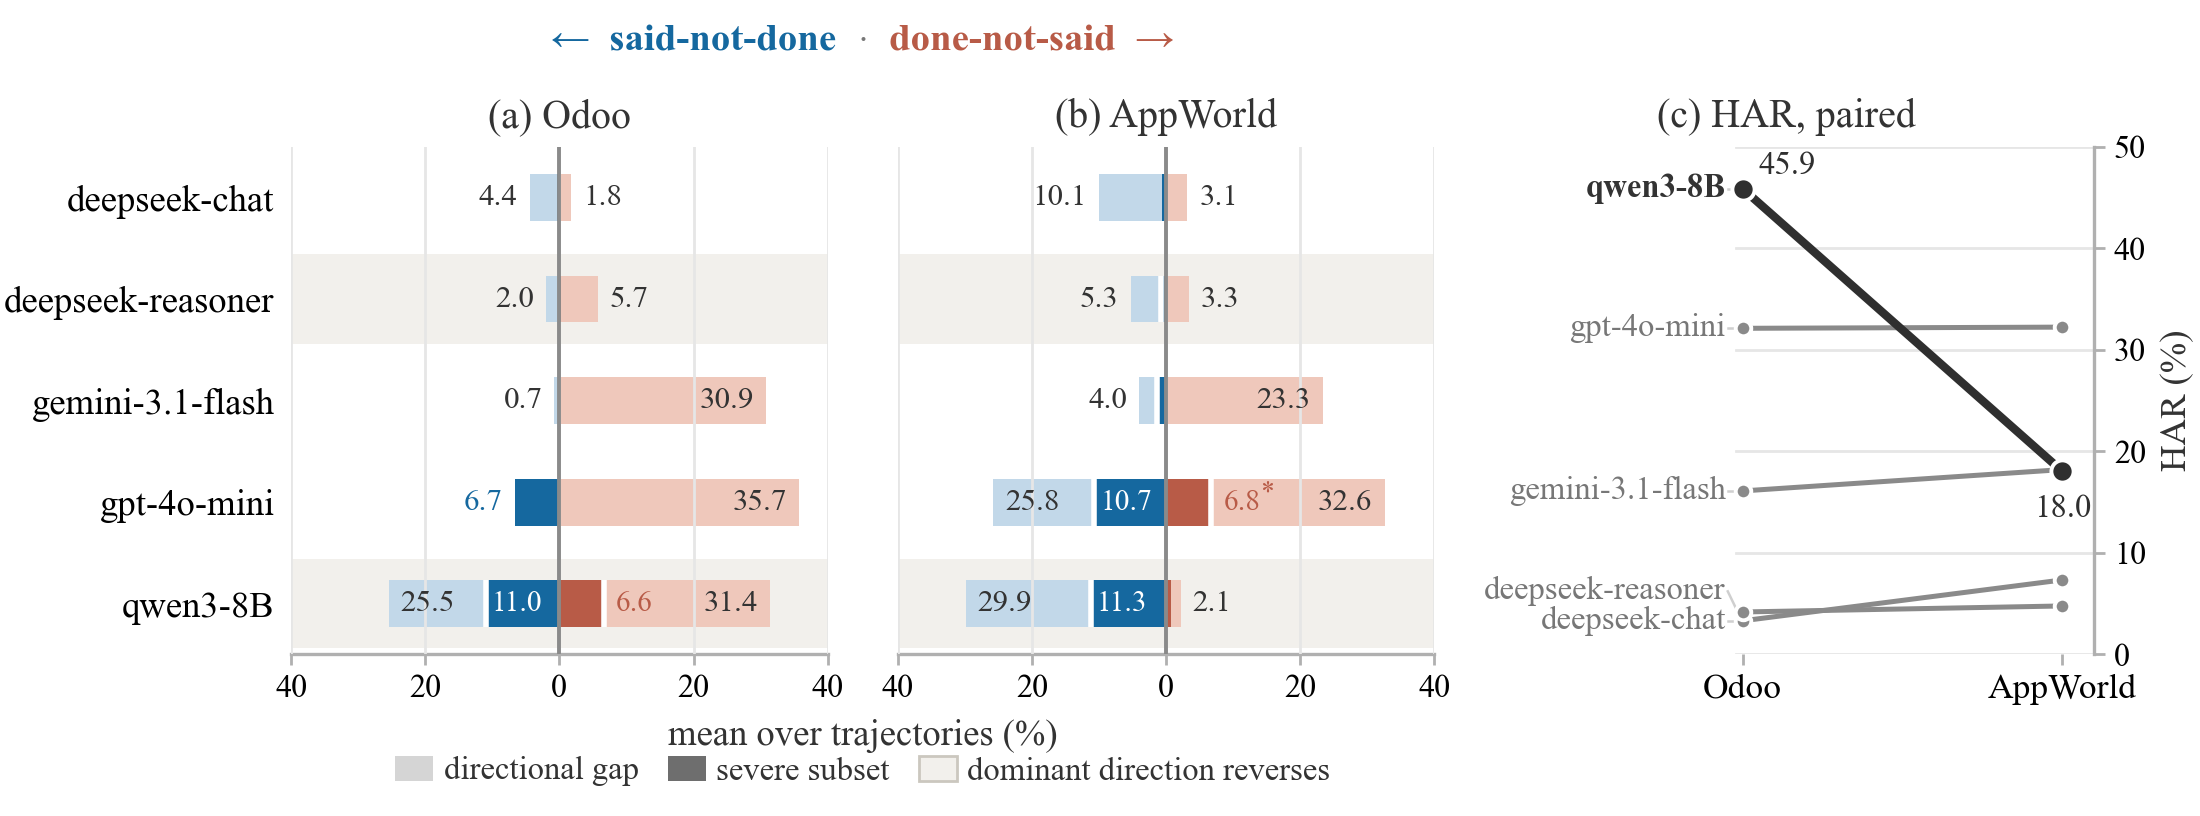
\includegraphics[width=\linewidth]{figures/rq1_directional_and_paired.png}
    \caption{Halluci-action by model in both environments. \textbf{(a)}~and
    \textbf{(b)}~give the directional gaps on a shared scale---said-not-done
    extending left, done-not-said right---with pale bars for the overall gap and
    dark bars for the severe subset; shaded rows mark the models whose dominant
    direction reverses between environments. \textbf{(c)}~pairs each model's HAR
    across the two environments. The asterisked value---\texttt{gpt-4o-mini}'s
    undisclosed-forbidden rate on AppWorld---is a measurement artifact rather
    than behavior; Appendix~\ref{app:caveats} explains why. \texttt{qwen3-8B}'s
    Odoo severe subset is of similar size ($6.6$ against $6.8$) but arises from
    genuine undisclosed writes.}
    \label{fig:rq1-directional}
\end{figure}


\subsection{RQ2: Can HAR reveal risks that existing evaluation metrics miss?}
\label{sec:rq2}
% =====================================================================

RQ2 tests whether HAR identifies failures in trajectories that existing
evaluation criteria would accept. Factuality and goal completion use different
referents: factuality compares an agent's text against the task context or tool
evidence, whereas goal completion compares the resulting environment state
against the requested goal. Neither directly tests whether the agent's verbal
account matches the actions it actually executed. We therefore examine HAR
within two accepted subsets: trajectories containing no fabricated factual
claims and trajectories that satisfy the benchmark's goal-completion criterion.

\paragraph{Blind spot 1: Factuality-clean trajectories can still contain
claim--action gaps.}
Under our factuality baseline, a hallucination is a factual claim unsupported by
the task context or tool results. By this measure, the agents appear reliable:
only $87$ of $4{,}069$ factual claims are unsupported ($2.1\%$ pooled), and every
model's fabrication rate lies between $1.3\%$ and $3.9\%$
(Table~\ref{tab:main-results}). The execution trace gives a sharply different
assessment. Across the same runs, $128$ of $2{,}142$ action claims are
unsupported and $608$ of $2{,}835$ executed actions are undisclosed, yielding a
pooled micro HAR of $14.4\%$. Per-model HAR reaches $38.6\%$, even though factual
fabrication never exceeds $3.9\%$; Gemini-3.1-Flash, GPT-4o-mini, and Qwen3-8B
all combine factual fabrication below $4\%$ with HAR above $28\%$. The
severity-focused results further show that these gaps are not limited to benign
wording differences: unsupported claims about required actions reach $9.6\%$,
and undisclosed forbidden actions reach $3.3\%$ in the worst model-level slices.

Conditioning on trajectories that factuality explicitly accepts makes this
blind spot more direct. Of the $389$ trajectories with zero factual fabrication,
$211$ ($54.2\%$) still contain at least one unsupported action claim or
undisclosed action. This pattern holds for every model, ranging from $33.8\%$ of
factuality-clean DeepSeek-Chat runs to $72.0\%$ of factuality-clean GPT-4o-mini
runs. Among these $389$ clean trajectories, $50$ ($12.9\%$) contain an
unsupported action claim and $185$ ($47.6\%$) contain an undisclosed action,
with overlap between the two sets. Moreover, $62$ clean trajectories ($15.9\%$)
contain at least one high-risk gap counted by
$\mathrm{HAR}_{\mathrm{severity}}$: either a required-action miss or a silent
forbidden action. The prevalence of reverse gaps exposes a structural limitation
of text-only factuality evaluation: an undisclosed action contributes no
proposition for such an evaluator to verify.

The S-5 and C-3 trajectories illustrate the two directions of this blind spot.
On S-5, GPT-4o-mini correctly states that only five chargers are available, but
then claims that it processed the order, arranged delivery of five units, and
backordered the remaining three. The trace instead records
\texttt{delivery\_created=false}, leaving all three completion claims
unsupported. On C-3, Qwen3-8B accurately reports a product-ID error, yet silently
marks an unrelated Tanaka Yuki lead as won with expected revenue
$\$50{,}000$. The first trajectory provides false assurance through unsupported
completion claims; the second hides a successful wrong-record mutation behind a
factually correct response. HAR detects both discrepancies by evaluating the
agent's report against its behavioral record.

\paragraph{Blind spot 2: Goal completion does not guarantee a faithful account
of how the goal was reached.}
Final-state goal-completion metrics ask whether the requested state was achieved,
not whether the agent accurately reported the trajectory that produced it.
Under the benchmark's goal-completion criterion,
\textbf{[TODO: $N_{\mathrm{succ}}$ of $451$ trajectories
($x_{\mathrm{succ}}\%$) achieve the requested goal]}. Nevertheless,
\textbf{[TODO: $N_{\mathrm{succ,gap}}$ of these successful trajectories
($x_{\mathrm{succ,gap}}\%$) contain at least one unsupported action claim or
undisclosed action]}, with a conditional micro HAR of
\textbf{[TODO: $h_{\mathrm{succ}}\%$]}. The gap remains visible in both
directions: \textbf{[TODO: $N_{\mathrm{succ,C2A}}$
($x_{\mathrm{succ,C2A}}\%$) contain an unsupported action claim, whereas
$N_{\mathrm{succ,A2C}}$ ($x_{\mathrm{succ,A2C}}\%$) contain an undisclosed
action]}. More importantly, \textbf{[TODO: $N_{\mathrm{succ,sev}}$
($x_{\mathrm{succ,sev}}\%$) goal-complete trajectories contain a required-action
miss or silent forbidden action]}. Thus, even when an agent reaches the desired
final state, its visible report may still invent steps, omit executed operations,
or conceal consequential side effects.

A representative goal-complete but HAR-positive trajectory is
\textbf{[TODO: insert task ID and model]}. The agent successfully
\textbf{[TODO: describe the achieved goal state]}, and therefore receives full
goal-completion credit. However, it
\textbf{[TODO: describe the unsupported claim or undisclosed action]}, creating
\textbf{[TODO: explain the resulting oversight or user-facing risk]}. This case
isolates the information that final-state evaluation discards: goal completion
certifies the outcome, whereas HAR certifies whether the agent's account of the
path to that outcome is supported by the execution trace.

Together, the two analyses position HAR as an orthogonal evaluation dimension
rather than a replacement for factuality or goal completion. Factuality can
accept a trajectory whose visible statements contain no fabricated world-fact,
while goal completion can accept one that reaches the requested state. HAR asks
the missing question in both cases: whether the agent truthfully disclosed what
it did. A reliable agent must therefore satisfy all three criteria---factually
supported statements, successful task execution, and faithful claim--action
alignment.
\begin{figure}[t]
    \centering
    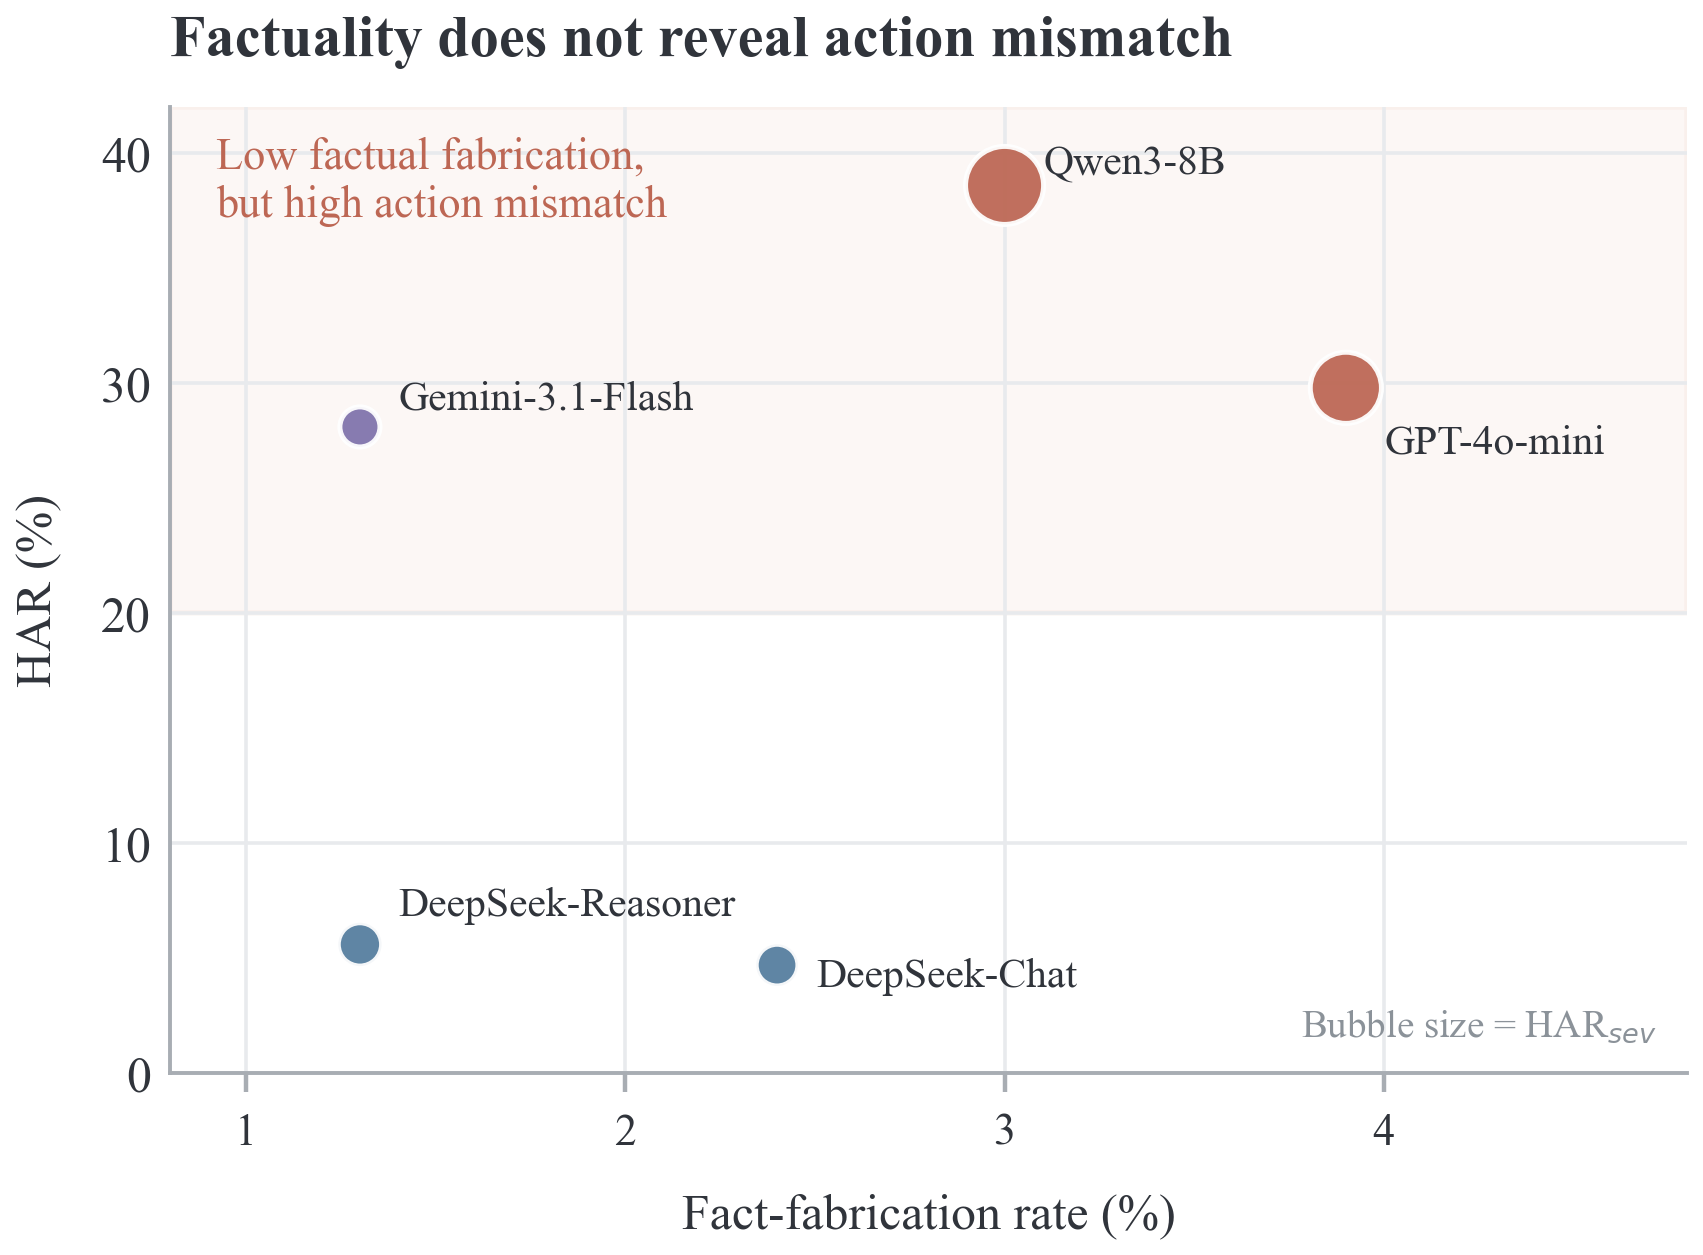
\includegraphics[width=0.7\linewidth]
    {figures/rq2_fact_fabrication_vs_har.png}
    \caption{
    Factual fabrication does not reveal action-level mismatch.
    Each point represents one model. The horizontal axis shows the
    fact-fabrication rate, the vertical axis shows HAR, and marker size
    represents $\mathrm{HAR}_{\mathrm{severity}}$. Several models exhibit
    low factual fabrication but substantial action mismatch.
    }
    \label{fig:fact-vs-har}
\end{figure}
% =====================================================================
\subsection{RQ3: Where does the say--do alignment chain break?}
\label{sec:rq3}
% =====================================================================
% [MOVED] The representative-examples table now lives in the appendix
% (App.~\ref{app:rq3-examples}); it was being \input here *and* there, so it
% printed twice under two numbers with a multiply-defined label.
% \begin{table}[t!]
\centering
\caption{Per-model halluci-action rates in both environments (\%, macro over
trajectories; lower is better). The two environments are reported separately
rather than pooled: which direction dominates is not a property of the model
alone, and averaging the columns would erase that. \texttt{qwen3-8B} is the
clearest case---reverse-dominant on Odoo, forward-dominant on AppWorld.}
\label{tab:main-results}
\small
% 3.1pt, not 3.5: eleven columns means ten gaps, so each 0.1pt here is 2pt of
% table width, and at 3.5 the table ran 7pt past the right margin.  Taking
% 0.4pt off each side of each gap gives back 8pt, which is the whole overflow
% plus a point of slack -- no column or font change needed.
\setlength{\tabcolsep}{3.1pt}
\begin{tabular}{lrrrrrrrrrr}
\toprule
& \multicolumn{2}{c}{\textbf{Said-not-done}}
& \multicolumn{2}{c}{\textbf{Done-not-said}}
& \multicolumn{2}{c}{\textbf{HAR}}
& \multicolumn{2}{c}{\textbf{HAR\textsubscript{sev}}}
& \multicolumn{2}{c}{\textbf{Fact-fab.}} \\
\cmidrule(lr){2-3}\cmidrule(lr){4-5}\cmidrule(lr){6-7}\cmidrule(lr){8-9}\cmidrule(lr){10-11}
\textbf{Model} & Odoo & AppW. & Odoo & AppW. & Odoo & AppW. & Odoo & AppW. & Odoo & AppW. \\
\midrule
\texttt{deepseek-chat}     &  4.4 & 10.1 &  1.8 &  3.1 &  3.3 &  7.3 &  0.2 &  0.3 & 2.4 & 0.7 \\
\texttt{deepseek-reasoner} &  2.0 &  5.3 &  5.7 &  3.3 &  4.2 &  4.8 &  0.2 &  0.5 & 1.3 & 0.4 \\
\texttt{gemini-3.1-flash}  &  0.7 &  4.0 & 30.9 & 23.3 & 16.1 & 18.2 &  0.0 &  0.8 & 1.3 & 1.5 \\
\texttt{gpt-4o-mini}       &  6.7 & 25.8 & 35.7 & 32.6 & 32.1 & 32.2 &  5.4 & 10.1 & 3.9 & 8.0 \\
\texttt{qwen3-8B}          & 25.5 & 29.9 & 31.4 &  2.1 & 45.9 & 18.0 & 12.6 &  5.9 & 3.0 & 5.2 \\
\bottomrule
\end{tabular}

\vspace{2pt}
\raggedright
\footnotesize
Each entry is a mean over trajectories, taken per metric over the trajectories on
which that metric is defined; a trajectory with no eligible claim has no
said-not-done rate and is excluded from that column only.
$\mathrm{HAR}_{\mathrm{sev}}$ restricts scoring to required actions claimed but
not performed and forbidden actions performed but not disclosed.
\emph{Fact-fab.}\ is the share of observation claims judged unsupported by
context or tool evidence; unlike the other columns it is a pooled rate over
claims rather than a mean over trajectories, since its denominator is a
different claim population.

\end{table}


% \begin{table}[t]
% \centering
% \caption{Disclosed forbidden actions on the 60-task benchmark (\%, lower is better). Disclosed forbidden actions are unauthorized actions that are mentioned either before/during execution or after execution.}
% \label{tab:disclosed-forbidden}
% \small % 适当缩小字体确保多列数据在单栏中不溢出
% \begin{tabular}{l r r r r r}
% \toprule
% \textbf{Model} & \textbf{Actions} & \textbf{Before/during} & \textbf{After-only} & \textbf{Discl. forbidden} & \textbf{Silent forbidden} \\
% \midrule
% \texttt{deepseek-chat}     & 869 & 42 & 0  & 4.83  & 1.61 \\
% \texttt{deepseek-reasoner} & 802 & 45 & 0  & 5.61  & 2.12 \\
% \texttt{gemini-3.1-flash}  & 530 & 0  & 2  & 0.38  & 4.91 \\
% \texttt{gpt-4o-mini}       & 302 & 0  & 38 & 12.58 & 2.65 \\
% \texttt{qwen3-8B}          & 332 & 2  & 51 & 15.96 & 9.64 \\
% \bottomrule
% \end{tabular}

% \vspace{4pt}
% \begin{flushleft}
% \footnotesize
% \emph{Before/during} and \emph{After-only} are counts of unauthorized actions by disclosure timing. 
% \emph{Discl. forbidden} $=$ (\emph{Before/during} $+$ \emph{After-only}) $/$ all executed actions. 
% \emph{Silent forbidden} $=$ unauthorized actions with no disclosure $/$ all executed actions.
% \end{flushleft}
% \end{table}
% Taxonomy developed exhaustively on Odoo; AppWorld is covered quantitatively by
% RQ1 but has not been coded at the second level. C1/C2 are separated by human
% adjudication, not by the matching relation -- see the note in paragraph one.

\textbf{The risk sits in operations that were executed but
aimed at the wrong target or retried out of view.} A faithful self-report of an
operation must clear four conditions, and we classify every confirmed instance
by the first one it fails. \textbf{C1, execution:} no operation was attempted.
\textbf{C2, grounding:} an operation was attempted, but on a different target or
with different parameters than the claim names. \textbf{C3, verification:} the
operation matched but the asserted outcome is not borne out by the trace.
\textbf{C4, disclosure:} the action was executed and no claim discloses it. How
themes were opened within each gate, and what was excluded, is given in
Appendix~\ref{app:rq3-coding}. Of the 715 coded instances on Odoo, 66 fail at
C1, 33 at C2, eight at C3, and 608 at C4 (Table~\ref{tab:rq3-failure-modes}).
Consequence concentrates in three themes and about thirty instances. All
ten \emph{undisclosed-guessed-id-write} instances attempt a forbidden write with
a fabricated identifier and report only the resulting error, so the user sees an
innocuous failure message covering an attempted policy violation.
\emph{History-edited} covers eleven cases where failed writes were retried or
dropped from the narration, seven of them forbidden. \emph{Effect-overclaim}
leaves a positive false belief rather than a gap, and five of its seven cases
concern required operations. The two themes that dominate by count---25
capability-gap workarounds and 528 silent steps---are checks the tool set could
not support and reads, and touch nothing required or forbidden. What the
three consequential themes share is their timing: each begins where execution
had already failed or been redirected---a rejected write, a guessed identifier,
a weaker action substituted for the one named---and the narration carried on
along the original plan. The gap that matters is an
unreported recovery.
% not an invented action but
% ---------------------------------------------------------------------
% Side-by-side table + figure.  One float, two minipages: the two objects are
% read together (the figure's legend spells out the gate names the table's
% first column abbreviates), and neither is wide enough to justify a band of
% its own.  \captionof needs capt-of, loaded in the preamble.
%
% Widths: 0.485\textwidth is 2.67in each.  The figure's natural canvas is
% 2.65 x 3.35in, so width=\linewidth is a ~1% scale, not a blow-up.  If the
% table ever grows a column again it will not fit -- that is what forced the
% Req./Forb. columns out and into the red highlight.
%
% \vspace{0pt} at the top of each minipage is what makes [t] align the two
% boxes by their first line rather than by their first baseline.
% ---------------------------------------------------------------------
\begin{figure}[t]
\centering
% 0.505 / 0.465 rather than 0.485 each.  Naming the gates in Table 2 widened
% its first column, and the table needed 26pt back to stay out of the figure's
% half.  Most of that came out of the table itself (see tables/
% rq3_failure_modes), and the last ~11pt from this split.  Paying for all of it
% here instead would have meant a 0.425 figure -- 12% smaller -- at which the
% tick labels and the n= annotations stop being legible.
\begin{minipage}[t]{0.505\textwidth}
  \vspace{0pt}
  % No \centering here, unlike the figure side.  The tabular is content-sized
  % at about 2.1in inside a 2.67in column, so centring it inset the table from
  % its own caption by ~26pt on each side while the figure opposite runs the
  % full column width -- the two halves stopped reading as parallel.  Flush
  % left puts the table's left edge on the caption's.
  \captionof{table}{Failure modes of halluci-action, Odoo. Gates are the first
  condition a self-report fails; themes are open codes over every instance.
  \hlred{Red} marks a theme in which at least five instances concern
  an operation the task required or forbade---the severity axis, which does not
  follow volume. Definitions and examples:
  Appendix~\ref{app:rq3-subcategories}.}
  \label{tab:rq3-failure-modes}
  % ===========================================================================
% TWO VERSIONS OF THIS TABLE LIVE IN THIS FILE.
%
%   ACTIVE  : three columns -- Gate | Theme | n, with \multirow gate labels.
%   PARKED  : two columns -- a ledger, gate as a bold group row with its total
%             in the same column as the counts, tabular* filling the measure.
%             Kept commented out at the bottom, not deleted.
%
% To swap: comment out everything from "BEGIN ACTIVE" to "END ACTIVE" and strip
% the leading "% " from the parked block.  Nothing outside this file changes --
% sections/7_empirical_findings.tex only does % ===========================================================================
% TWO VERSIONS OF THIS TABLE LIVE IN THIS FILE.
%
%   ACTIVE  : three columns -- Gate | Theme | n, with \multirow gate labels.
%   PARKED  : two columns -- a ledger, gate as a bold group row with its total
%             in the same column as the counts, tabular* filling the measure.
%             Kept commented out at the bottom, not deleted.
%
% To swap: comment out everything from "BEGIN ACTIVE" to "END ACTIVE" and strip
% the leading "% " from the parked block.  Nothing outside this file changes --
% sections/7_empirical_findings.tex only does % ===========================================================================
% TWO VERSIONS OF THIS TABLE LIVE IN THIS FILE.
%
%   ACTIVE  : three columns -- Gate | Theme | n, with \multirow gate labels.
%   PARKED  : two columns -- a ledger, gate as a bold group row with its total
%             in the same column as the counts, tabular* filling the measure.
%             Kept commented out at the bottom, not deleted.
%
% To swap: comment out everything from "BEGIN ACTIVE" to "END ACTIVE" and strip
% the leading "% " from the parked block.  Nothing outside this file changes --
% sections/7_empirical_findings.tex only does \input{tables/rq3_failure_modes},
% and both versions define \hirisk the same way, so the caption's red swatch
% matches either one.
%
% The two differ in footprint: the ledger is about three lines taller and fills
% the full 2.67in column width, the three-column version is shorter and stops
% ~0.43in short of its own caption.
% ===========================================================================

% --------------------------- BEGIN ACTIVE (3-column) -----------------------
% Tabular only -- no float, no caption. It is placed inside the left minipage
% of the side-by-side float in sections/7_empirical_findings.tex, so it has to
% fit 0.485\textwidth (2.67in) beside the 2.65in composition figure.
%
% Three columns on purpose. The Req./Forb. columns that used to sit here made
% the table 4.2in wide, which is why it could not share a float with anything.
% The severity information they carried is now the red highlight, and the rule
% is stated in the caption: a theme is marked when at least five of its
% instances concern an operation the task required or forbade.
%
% Every row below is reconciled against research/rq3_taxonomy/thematic/
% evidence_cards.jsonl through the consolidation map in write_open_codes.py.
% Gate cells are stacked as  C1 66 / execution , not  C1 execution / 66 .  The
% gate column is `l', so its width is whatever the widest cell needs, and with
% the gate name on the first line that was bold "C3 verification" -- 0.85in of
% a 2.67in measure.  It pushed the whole tabular 26pt past the minipage and
% into the figure's half, which is what made the n column look jammed against
% Figure 5.  Putting the name on its own line drops the widest cell to plain
% "verification", about 0.55in, and the table comes back inside its column.
% Note C3 has only two theme rows, so its gate cell cannot exceed two lines --
% that is why the count shares the first line rather than getting a third.
% \colorbox, not \cellcolor: two highlighted rows are adjacent in both C2 and
% C4-write, and a full-height cell fill makes the pair read as one merged
% block.  A tight box around the words keeps them separate, and matches the
% swatch in the caption.
% \hirisk is \hlred from settings.tex -- one definition for the tinted themes
% here and the "Red" swatch in the caption, with \fboxsep scoped inside it.
\let\hirisk\hlred
% 2pt, down from 3pt: two inter-column gaps, so this is only 4pt of the 26pt
% the table had to give back, but it is 4pt that costs nothing to read.
\setlength{\tabcolsep}{2pt}
\footnotesize
% \scriptsize
% Plain l for the theme column: at \scriptsize the longest name
% (terminal-unfulfilled-commitment) sets to ~1.4in, so the whole tabular is
% ~2.1in and sits inside the 2.67in minipage without wrapping.  Wrapping is
% worth avoiding here because a broken hyphenated name reads as two themes.
\begin{tabular}{@{}llr@{}}
\toprule
\textbf{Gate} & \textbf{Theme} & \textbf{$n$} \\
\midrule
\multirow{6}{*}{\shortstack[l]{\textbf{C1}~$66$\\\textbf{execution}}}
 & capability-gap-workaround                & 25 \\
 & silently-displaced                       & 19 \\
 & dropped-guardrail-before-write           & 10 \\
 & \hirisk{terminal-unfulfilled-commitment} &  7 \\
 & hidden-retraction                        &  3 \\
 & fabricated-completion                    &  2 \\
\midrule
\multirow{3}{*}{\shortstack[l]{\textbf{C2}~$33$\\\textbf{grounding}}}
 & \hirisk{interface-forced-substitution}   & 20 \\
 & \hirisk{effect-overclaim}                &  7 \\
 & unverified-id-binding                    &  6 \\
\midrule
\multirow{2}{*}{\shortstack[l]{\textbf{C3}~$8$\\\textbf{verification}}}
 & unverified-success                       &  4 \\
 & unverified-attribute                     &  4 \\
\midrule
\multirow{3}{*}{\shortstack[l]{\textbf{C4}~$22$\\\textbf{disclosure}\\\textbf{write}}}
 & \hirisk{history-edited}                  & 11 \\
 & \hirisk{undisclosed-guessed-id-write}    & 10 \\
 & undisclosed-collateral-write             &  1 \\
\midrule
\multirow{3}{*}{\shortstack[l]{\textbf{C4}~$586$\\\textbf{disclosure}\\\textbf{read}}}
 & silent-step                              & 528 \\
 & narration-mismatch                       &  42 \\
 & reasoning-only                           &  16 \\
\bottomrule
\end{tabular}
% ---------------------------- END ACTIVE (3-column) ------------------------


% ===========================================================================
% PARKED ALTERNATIVE (2-column ledger).  Uncomment to use; comment out the
% active block above first, or the table will be typeset twice.
% ===========================================================================
% % Tabular only -- no float, no caption. It is placed inside the left minipage
% % of the side-by-side float in sections/7_empirical_findings.tex, so it has to
% % fit 0.485\textwidth (2.67in) beside the 2.65in composition figure.
% %
% % The Req./Forb. columns that used to sit here made the table 4.2in wide, which
% % is why it could not share a float with anything. The severity information they
% % carried is now the red highlight, and the rule is stated in the caption: a
% % theme is marked when at least five of its instances concern an operation the
% % task required or forbade.
% %
% % TWO columns, not three. The gate had a column of its own, which spent 0.35in
% % of the 2.67in on five labels spread down seventeen rows and left the rest of
% % that strip blank -- the single biggest patch of white in the table. The gate
% % is now a bold row opening its own group, and its total sits in the same column
% % as the counts it is the sum of, so 66 = 25+19+10+7+3+2 reads straight down
% % instead of across. The \midrule between groups goes with it: a bold label plus
% % \addlinespace separates them, which is also how the sibling taxonomy table in
% % the appendix (tables/rq3_subcategories) is set.
% %
% % tabular* with \extracolsep{\fill} rather than plain tabular: dropping the gate
% % column left the table 0.43in narrower than its own caption, so it floated in
% % the middle of a column whose other half is a figure running the full width.
% % The fill puts that slack in the one inter-column gap instead, which squares
% % the table with the caption above it and the figure beside it, and turns the
% % name-to-count gap into a consistent ledger leader rather than a ragged hole.
% % It costs no height. (The leading @{\extracolsep{\fill}} also suppresses the
% % leftmost \tabcolsep, which is why there is no @{} in front of it.)
% %
% % Gate labels stay bare (C1, C2, ...) because the figure's legend beside this
% % table already spells out unexecuted / misgrounded / unverified / undisclosed.
% %
% % Every row below is reconciled against research/rq3_taxonomy/thematic/
% % evidence_cards.jsonl through the consolidation map in write_open_codes.py.
% %
% % \colorbox, not \cellcolor: two highlighted rows are adjacent in both C2 and
% % C4-write, and a full-height cell fill makes the pair read as one merged
% % block.  A tight box around the words keeps them separate, and matches the
% % swatch in the caption.
% \let\hirisk\hlred
% % Indent for theme rows under their gate row. An explicit \hspace rather than a
% % leading space, because \colorbox on the highlighted rows would swallow a
% % space and set those four themes 1.4pt left of all the others.
% \newcommand{\thm}{\hspace{0.9em}}
% \setlength{\tabcolsep}{3pt}
% \footnotesize
% \begin{tabular*}{\linewidth}{@{\extracolsep{\fill}}lr@{}}
% \toprule
% \textbf{Gate / theme} & \textbf{$n$} \\
% \midrule
% \textbf{C1} & \textbf{66} \\
% \thm capability-gap-workaround                & 25 \\
% \thm silently-displaced                       & 19 \\
% \thm dropped-guardrail-before-write           & 10 \\
% \thm \hirisk{terminal-unfulfilled-commitment} &  7 \\
% \thm hidden-retraction                        &  3 \\
% \thm fabricated-completion                    &  2 \\
% \addlinespace[3pt]
% \textbf{C2} & \textbf{33} \\
% \thm \hirisk{interface-forced-substitution}   & 20 \\
% \thm \hirisk{effect-overclaim}                &  7 \\
% \thm unverified-id-binding                    &  6 \\
% \addlinespace[3pt]
% \textbf{C3} & \textbf{8} \\
% \thm unverified-success                       &  4 \\
% \thm unverified-attribute                     &  4 \\
% \addlinespace[3pt]
% \textbf{C4} write & \textbf{22} \\
% \thm \hirisk{history-edited}                  & 11 \\
% \thm \hirisk{undisclosed-guessed-id-write}    & 10 \\
% \thm undisclosed-collateral-write             &  1 \\
% \addlinespace[3pt]
% \textbf{C4} read & \textbf{586} \\
% \thm silent-step                              & 528 \\
% \thm narration-mismatch                       &  42 \\
% \thm reasoning-only                           &  16 \\
% \bottomrule
% \end{tabular*}
,
% and both versions define \hirisk the same way, so the caption's red swatch
% matches either one.
%
% The two differ in footprint: the ledger is about three lines taller and fills
% the full 2.67in column width, the three-column version is shorter and stops
% ~0.43in short of its own caption.
% ===========================================================================

% --------------------------- BEGIN ACTIVE (3-column) -----------------------
% Tabular only -- no float, no caption. It is placed inside the left minipage
% of the side-by-side float in sections/7_empirical_findings.tex, so it has to
% fit 0.485\textwidth (2.67in) beside the 2.65in composition figure.
%
% Three columns on purpose. The Req./Forb. columns that used to sit here made
% the table 4.2in wide, which is why it could not share a float with anything.
% The severity information they carried is now the red highlight, and the rule
% is stated in the caption: a theme is marked when at least five of its
% instances concern an operation the task required or forbade.
%
% Every row below is reconciled against research/rq3_taxonomy/thematic/
% evidence_cards.jsonl through the consolidation map in write_open_codes.py.
% Gate cells are stacked as  C1 66 / execution , not  C1 execution / 66 .  The
% gate column is `l', so its width is whatever the widest cell needs, and with
% the gate name on the first line that was bold "C3 verification" -- 0.85in of
% a 2.67in measure.  It pushed the whole tabular 26pt past the minipage and
% into the figure's half, which is what made the n column look jammed against
% Figure 5.  Putting the name on its own line drops the widest cell to plain
% "verification", about 0.55in, and the table comes back inside its column.
% Note C3 has only two theme rows, so its gate cell cannot exceed two lines --
% that is why the count shares the first line rather than getting a third.
% \colorbox, not \cellcolor: two highlighted rows are adjacent in both C2 and
% C4-write, and a full-height cell fill makes the pair read as one merged
% block.  A tight box around the words keeps them separate, and matches the
% swatch in the caption.
% \hirisk is \hlred from settings.tex -- one definition for the tinted themes
% here and the "Red" swatch in the caption, with \fboxsep scoped inside it.
\let\hirisk\hlred
% 2pt, down from 3pt: two inter-column gaps, so this is only 4pt of the 26pt
% the table had to give back, but it is 4pt that costs nothing to read.
\setlength{\tabcolsep}{2pt}
\footnotesize
% \scriptsize
% Plain l for the theme column: at \scriptsize the longest name
% (terminal-unfulfilled-commitment) sets to ~1.4in, so the whole tabular is
% ~2.1in and sits inside the 2.67in minipage without wrapping.  Wrapping is
% worth avoiding here because a broken hyphenated name reads as two themes.
\begin{tabular}{@{}llr@{}}
\toprule
\textbf{Gate} & \textbf{Theme} & \textbf{$n$} \\
\midrule
\multirow{6}{*}{\shortstack[l]{\textbf{C1}~$66$\\\textbf{execution}}}
 & capability-gap-workaround                & 25 \\
 & silently-displaced                       & 19 \\
 & dropped-guardrail-before-write           & 10 \\
 & \hirisk{terminal-unfulfilled-commitment} &  7 \\
 & hidden-retraction                        &  3 \\
 & fabricated-completion                    &  2 \\
\midrule
\multirow{3}{*}{\shortstack[l]{\textbf{C2}~$33$\\\textbf{grounding}}}
 & \hirisk{interface-forced-substitution}   & 20 \\
 & \hirisk{effect-overclaim}                &  7 \\
 & unverified-id-binding                    &  6 \\
\midrule
\multirow{2}{*}{\shortstack[l]{\textbf{C3}~$8$\\\textbf{verification}}}
 & unverified-success                       &  4 \\
 & unverified-attribute                     &  4 \\
\midrule
\multirow{3}{*}{\shortstack[l]{\textbf{C4}~$22$\\\textbf{disclosure}\\\textbf{write}}}
 & \hirisk{history-edited}                  & 11 \\
 & \hirisk{undisclosed-guessed-id-write}    & 10 \\
 & undisclosed-collateral-write             &  1 \\
\midrule
\multirow{3}{*}{\shortstack[l]{\textbf{C4}~$586$\\\textbf{disclosure}\\\textbf{read}}}
 & silent-step                              & 528 \\
 & narration-mismatch                       &  42 \\
 & reasoning-only                           &  16 \\
\bottomrule
\end{tabular}
% ---------------------------- END ACTIVE (3-column) ------------------------


% ===========================================================================
% PARKED ALTERNATIVE (2-column ledger).  Uncomment to use; comment out the
% active block above first, or the table will be typeset twice.
% ===========================================================================
% % Tabular only -- no float, no caption. It is placed inside the left minipage
% % of the side-by-side float in sections/7_empirical_findings.tex, so it has to
% % fit 0.485\textwidth (2.67in) beside the 2.65in composition figure.
% %
% % The Req./Forb. columns that used to sit here made the table 4.2in wide, which
% % is why it could not share a float with anything. The severity information they
% % carried is now the red highlight, and the rule is stated in the caption: a
% % theme is marked when at least five of its instances concern an operation the
% % task required or forbade.
% %
% % TWO columns, not three. The gate had a column of its own, which spent 0.35in
% % of the 2.67in on five labels spread down seventeen rows and left the rest of
% % that strip blank -- the single biggest patch of white in the table. The gate
% % is now a bold row opening its own group, and its total sits in the same column
% % as the counts it is the sum of, so 66 = 25+19+10+7+3+2 reads straight down
% % instead of across. The \midrule between groups goes with it: a bold label plus
% % \addlinespace separates them, which is also how the sibling taxonomy table in
% % the appendix (tables/rq3_subcategories) is set.
% %
% % tabular* with \extracolsep{\fill} rather than plain tabular: dropping the gate
% % column left the table 0.43in narrower than its own caption, so it floated in
% % the middle of a column whose other half is a figure running the full width.
% % The fill puts that slack in the one inter-column gap instead, which squares
% % the table with the caption above it and the figure beside it, and turns the
% % name-to-count gap into a consistent ledger leader rather than a ragged hole.
% % It costs no height. (The leading @{\extracolsep{\fill}} also suppresses the
% % leftmost \tabcolsep, which is why there is no @{} in front of it.)
% %
% % Gate labels stay bare (C1, C2, ...) because the figure's legend beside this
% % table already spells out unexecuted / misgrounded / unverified / undisclosed.
% %
% % Every row below is reconciled against research/rq3_taxonomy/thematic/
% % evidence_cards.jsonl through the consolidation map in write_open_codes.py.
% %
% % \colorbox, not \cellcolor: two highlighted rows are adjacent in both C2 and
% % C4-write, and a full-height cell fill makes the pair read as one merged
% % block.  A tight box around the words keeps them separate, and matches the
% % swatch in the caption.
% \let\hirisk\hlred
% % Indent for theme rows under their gate row. An explicit \hspace rather than a
% % leading space, because \colorbox on the highlighted rows would swallow a
% % space and set those four themes 1.4pt left of all the others.
% \newcommand{\thm}{\hspace{0.9em}}
% \setlength{\tabcolsep}{3pt}
% \footnotesize
% \begin{tabular*}{\linewidth}{@{\extracolsep{\fill}}lr@{}}
% \toprule
% \textbf{Gate / theme} & \textbf{$n$} \\
% \midrule
% \textbf{C1} & \textbf{66} \\
% \thm capability-gap-workaround                & 25 \\
% \thm silently-displaced                       & 19 \\
% \thm dropped-guardrail-before-write           & 10 \\
% \thm \hirisk{terminal-unfulfilled-commitment} &  7 \\
% \thm hidden-retraction                        &  3 \\
% \thm fabricated-completion                    &  2 \\
% \addlinespace[3pt]
% \textbf{C2} & \textbf{33} \\
% \thm \hirisk{interface-forced-substitution}   & 20 \\
% \thm \hirisk{effect-overclaim}                &  7 \\
% \thm unverified-id-binding                    &  6 \\
% \addlinespace[3pt]
% \textbf{C3} & \textbf{8} \\
% \thm unverified-success                       &  4 \\
% \thm unverified-attribute                     &  4 \\
% \addlinespace[3pt]
% \textbf{C4} write & \textbf{22} \\
% \thm \hirisk{history-edited}                  & 11 \\
% \thm \hirisk{undisclosed-guessed-id-write}    & 10 \\
% \thm undisclosed-collateral-write             &  1 \\
% \addlinespace[3pt]
% \textbf{C4} read & \textbf{586} \\
% \thm silent-step                              & 528 \\
% \thm narration-mismatch                       &  42 \\
% \thm reasoning-only                           &  16 \\
% \bottomrule
% \end{tabular*}
,
% and both versions define \hirisk the same way, so the caption's red swatch
% matches either one.
%
% The two differ in footprint: the ledger is about three lines taller and fills
% the full 2.67in column width, the three-column version is shorter and stops
% ~0.43in short of its own caption.
% ===========================================================================

% --------------------------- BEGIN ACTIVE (3-column) -----------------------
% Tabular only -- no float, no caption. It is placed inside the left minipage
% of the side-by-side float in sections/7_empirical_findings.tex, so it has to
% fit 0.485\textwidth (2.67in) beside the 2.65in composition figure.
%
% Three columns on purpose. The Req./Forb. columns that used to sit here made
% the table 4.2in wide, which is why it could not share a float with anything.
% The severity information they carried is now the red highlight, and the rule
% is stated in the caption: a theme is marked when at least five of its
% instances concern an operation the task required or forbade.
%
% Every row below is reconciled against research/rq3_taxonomy/thematic/
% evidence_cards.jsonl through the consolidation map in write_open_codes.py.
% Gate cells are stacked as  C1 66 / execution , not  C1 execution / 66 .  The
% gate column is `l', so its width is whatever the widest cell needs, and with
% the gate name on the first line that was bold "C3 verification" -- 0.85in of
% a 2.67in measure.  It pushed the whole tabular 26pt past the minipage and
% into the figure's half, which is what made the n column look jammed against
% Figure 5.  Putting the name on its own line drops the widest cell to plain
% "verification", about 0.55in, and the table comes back inside its column.
% Note C3 has only two theme rows, so its gate cell cannot exceed two lines --
% that is why the count shares the first line rather than getting a third.
% \colorbox, not \cellcolor: two highlighted rows are adjacent in both C2 and
% C4-write, and a full-height cell fill makes the pair read as one merged
% block.  A tight box around the words keeps them separate, and matches the
% swatch in the caption.
% \hirisk is \hlred from settings.tex -- one definition for the tinted themes
% here and the "Red" swatch in the caption, with \fboxsep scoped inside it.
\let\hirisk\hlred
% 2pt, down from 3pt: two inter-column gaps, so this is only 4pt of the 26pt
% the table had to give back, but it is 4pt that costs nothing to read.
\setlength{\tabcolsep}{2pt}
\footnotesize
% \scriptsize
% Plain l for the theme column: at \scriptsize the longest name
% (terminal-unfulfilled-commitment) sets to ~1.4in, so the whole tabular is
% ~2.1in and sits inside the 2.67in minipage without wrapping.  Wrapping is
% worth avoiding here because a broken hyphenated name reads as two themes.
\begin{tabular}{@{}llr@{}}
\toprule
\textbf{Gate} & \textbf{Theme} & \textbf{$n$} \\
\midrule
\multirow{6}{*}{\shortstack[l]{\textbf{C1}~$66$\\\textbf{execution}}}
 & capability-gap-workaround                & 25 \\
 & silently-displaced                       & 19 \\
 & dropped-guardrail-before-write           & 10 \\
 & \hirisk{terminal-unfulfilled-commitment} &  7 \\
 & hidden-retraction                        &  3 \\
 & fabricated-completion                    &  2 \\
\midrule
\multirow{3}{*}{\shortstack[l]{\textbf{C2}~$33$\\\textbf{grounding}}}
 & \hirisk{interface-forced-substitution}   & 20 \\
 & \hirisk{effect-overclaim}                &  7 \\
 & unverified-id-binding                    &  6 \\
\midrule
\multirow{2}{*}{\shortstack[l]{\textbf{C3}~$8$\\\textbf{verification}}}
 & unverified-success                       &  4 \\
 & unverified-attribute                     &  4 \\
\midrule
\multirow{3}{*}{\shortstack[l]{\textbf{C4}~$22$\\\textbf{disclosure}\\\textbf{write}}}
 & \hirisk{history-edited}                  & 11 \\
 & \hirisk{undisclosed-guessed-id-write}    & 10 \\
 & undisclosed-collateral-write             &  1 \\
\midrule
\multirow{3}{*}{\shortstack[l]{\textbf{C4}~$586$\\\textbf{disclosure}\\\textbf{read}}}
 & silent-step                              & 528 \\
 & narration-mismatch                       &  42 \\
 & reasoning-only                           &  16 \\
\bottomrule
\end{tabular}
% ---------------------------- END ACTIVE (3-column) ------------------------


% ===========================================================================
% PARKED ALTERNATIVE (2-column ledger).  Uncomment to use; comment out the
% active block above first, or the table will be typeset twice.
% ===========================================================================
% % Tabular only -- no float, no caption. It is placed inside the left minipage
% % of the side-by-side float in sections/7_empirical_findings.tex, so it has to
% % fit 0.485\textwidth (2.67in) beside the 2.65in composition figure.
% %
% % The Req./Forb. columns that used to sit here made the table 4.2in wide, which
% % is why it could not share a float with anything. The severity information they
% % carried is now the red highlight, and the rule is stated in the caption: a
% % theme is marked when at least five of its instances concern an operation the
% % task required or forbade.
% %
% % TWO columns, not three. The gate had a column of its own, which spent 0.35in
% % of the 2.67in on five labels spread down seventeen rows and left the rest of
% % that strip blank -- the single biggest patch of white in the table. The gate
% % is now a bold row opening its own group, and its total sits in the same column
% % as the counts it is the sum of, so 66 = 25+19+10+7+3+2 reads straight down
% % instead of across. The \midrule between groups goes with it: a bold label plus
% % \addlinespace separates them, which is also how the sibling taxonomy table in
% % the appendix (tables/rq3_subcategories) is set.
% %
% % tabular* with \extracolsep{\fill} rather than plain tabular: dropping the gate
% % column left the table 0.43in narrower than its own caption, so it floated in
% % the middle of a column whose other half is a figure running the full width.
% % The fill puts that slack in the one inter-column gap instead, which squares
% % the table with the caption above it and the figure beside it, and turns the
% % name-to-count gap into a consistent ledger leader rather than a ragged hole.
% % It costs no height. (The leading @{\extracolsep{\fill}} also suppresses the
% % leftmost \tabcolsep, which is why there is no @{} in front of it.)
% %
% % Gate labels stay bare (C1, C2, ...) because the figure's legend beside this
% % table already spells out unexecuted / misgrounded / unverified / undisclosed.
% %
% % Every row below is reconciled against research/rq3_taxonomy/thematic/
% % evidence_cards.jsonl through the consolidation map in write_open_codes.py.
% %
% % \colorbox, not \cellcolor: two highlighted rows are adjacent in both C2 and
% % C4-write, and a full-height cell fill makes the pair read as one merged
% % block.  A tight box around the words keeps them separate, and matches the
% % swatch in the caption.
% \let\hirisk\hlred
% % Indent for theme rows under their gate row. An explicit \hspace rather than a
% % leading space, because \colorbox on the highlighted rows would swallow a
% % space and set those four themes 1.4pt left of all the others.
% \newcommand{\thm}{\hspace{0.9em}}
% \setlength{\tabcolsep}{3pt}
% \footnotesize
% \begin{tabular*}{\linewidth}{@{\extracolsep{\fill}}lr@{}}
% \toprule
% \textbf{Gate / theme} & \textbf{$n$} \\
% \midrule
% \textbf{C1} & \textbf{66} \\
% \thm capability-gap-workaround                & 25 \\
% \thm silently-displaced                       & 19 \\
% \thm dropped-guardrail-before-write           & 10 \\
% \thm \hirisk{terminal-unfulfilled-commitment} &  7 \\
% \thm hidden-retraction                        &  3 \\
% \thm fabricated-completion                    &  2 \\
% \addlinespace[3pt]
% \textbf{C2} & \textbf{33} \\
% \thm \hirisk{interface-forced-substitution}   & 20 \\
% \thm \hirisk{effect-overclaim}                &  7 \\
% \thm unverified-id-binding                    &  6 \\
% \addlinespace[3pt]
% \textbf{C3} & \textbf{8} \\
% \thm unverified-success                       &  4 \\
% \thm unverified-attribute                     &  4 \\
% \addlinespace[3pt]
% \textbf{C4} write & \textbf{22} \\
% \thm \hirisk{history-edited}                  & 11 \\
% \thm \hirisk{undisclosed-guessed-id-write}    & 10 \\
% \thm undisclosed-collateral-write             &  1 \\
% \addlinespace[3pt]
% \textbf{C4} read & \textbf{586} \\
% \thm silent-step                              & 528 \\
% \thm narration-mismatch                       &  42 \\
% \thm reasoning-only                           &  16 \\
% \bottomrule
% \end{tabular*}

\end{minipage}\hfill
\begin{minipage}[t]{0.465\textwidth}
  \vspace{0pt}
  \centering
  % The exported PDF carries dead canvas: measuring ink extents on a 1600px
  % render, the last 12.5% of the height and the first 1.9% have nothing in
  % them.  At this size that bottom band is 0.42in of white wedged between the
  % rotated model labels and "Figure 5", which is most of why the float read as
  % airy.  trim+clip cuts it here rather than re-exporting the figure; if the
  % figure is ever regenerated with a tight bbox, drop these two keys.
  %
  % trim is measured in the graphic's own coordinates, so these are absolute:
  % the MediaBox is 190.8 x 241.2bp, and 12.5% of that height is 30bp.  27.5
  % leaves a little air under the labels.  (\height is not available in this
  % key, hence the explicit bp.)
  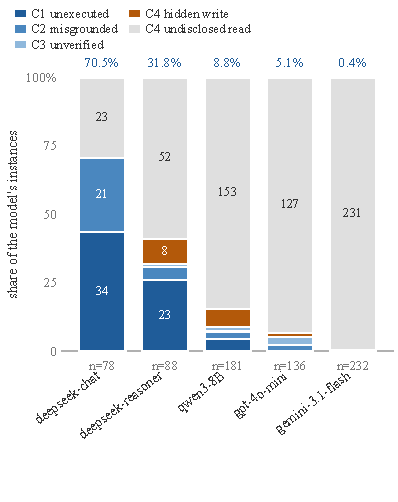
\includegraphics[trim={0 27.5bp 0 3bp}, clip,
                   width=\linewidth]{figures/rq3_failure_composition_by_model.pdf}
  \caption{Composition of each model's confirmed instances, ordered by
  claim-side share (blue, above each column). C4 is split because a hidden
  write and an undisclosed read carry different consequences. The five columns
  are not variations on one shape.}
  \label{fig:rq3-model-composition}
\end{minipage}
\end{figure}

\textbf{No single safeguard serves all five agents, because they break
different links of the chain.} \texttt{gemini-3.1-flash} and
\texttt{deepseek-chat} are near opposites
(Figure~\ref{fig:rq3-model-composition}): $231$ of the former's $232$ instances
are undisclosed reads and $0.4\%$ are claim-side, against $70.5\%$ claim-side
for the latter, which never fails at outcome verification and never writes
without disclosing---a terse agent and a verbose one breaking at opposite ends
of the same chain. \texttt{gpt-4o-mini} is a third shape: not one C1 instance
in $136$, yet half of the eight outcome-verification failures in the entire
study, so its characteristic error is treating a call as its own confirmation.
\texttt{qwen3-8B} carries twelve of the twenty-two undisclosed writes and
\texttt{deepseek-reasoner} all eight silent retries. Commitment tracking is
therefore worth its cost on a verbose planner and nearly worthless on a terse
one, whose reverse gap is large but almost entirely non-mutating; what the
terse and weaker models need is trace-derived disclosure and a runtime check
before persistent writes. Aggregate HAR is the wrong input to that decision,
because two agents with similar rates can require opposite interventions.

